\documentclass[pdflatex,compress]{beamer}

%\usetheme[dark,framenumber,totalframenumber]{ElektroITK}
\usetheme[darktitle,framenumber,totalframenumber]{ElektroITK}
\usepackage{graphicx}
\usepackage{multicol}

\title{Data Communications}

\subtitle{Chapter 1 - Introduction}

\author{Mifta Nur Farid}

\date{24 January 2024}

\begin{document}

\maketitle

\begin{frame}
	\frametitle{Contemporary Data Comms}
	\begin{itemize}
		\item trends
		\begin{itemize}
			\item traffic growth at a high \& steady rate
			\item development of new services
			\item advances in technology
		\end{itemize}
		\item significant change in requirements
		\begin{itemize}
			\item emergence of high-speed LANs
			\item corporate WAN needs
			\item digital electronics
		\end{itemize}
	\end{itemize}
\end{frame}

\begin{frame}
	\frametitle{A Communications Model}
	\begin{figure}
		\centering
		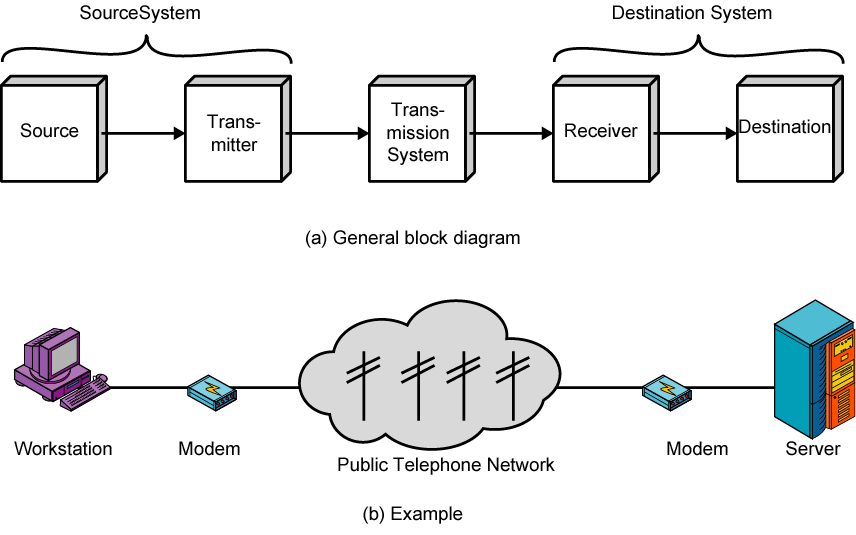
\includegraphics[width=\linewidth]{img/img01}
		\label{fig:img01}
	\end{figure}
\end{frame}

\begin{frame}
	\frametitle{Communications Tasks}
	\begin{figure}
		\centering
		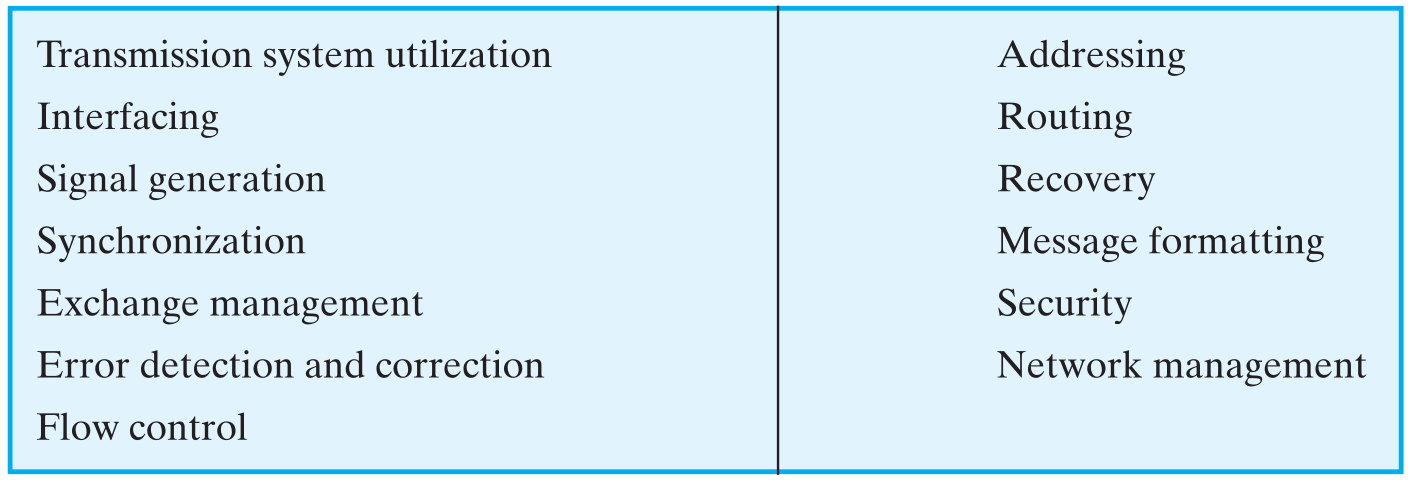
\includegraphics[width=\linewidth]{img/img02}
		\label{fig:img02}
	\end{figure}
\end{frame}

\begin{frame}
	\frametitle{Data Communications Model}
	\begin{figure}
		\centering
		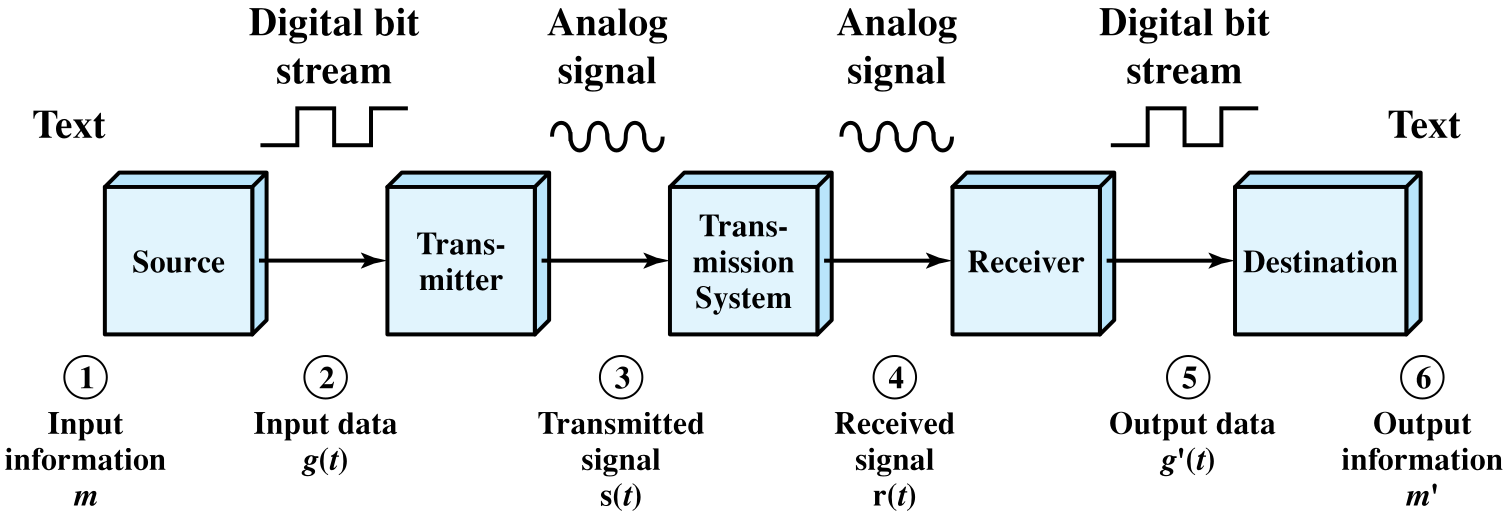
\includegraphics[width=\linewidth]{img/img03}
		\label{fig:img03}
	\end{figure}
\end{frame}

\begin{frame}
	\frametitle{Transmission Medium}
	\begin{itemize}
		\item selection is a basic choice
		\begin{itemize}
			\item internal use entirely up to business
			\item long-distance links made by carrier
		\end{itemize}
		\item rapid technology advances change mix
		\begin{itemize}
			\item fiber optic
			\item wireless
		\end{itemize}
		\item transmission costs still high
		\item hence interest in efficiency improvements
	\end{itemize}
\end{frame}

\begin{frame}
	\frametitle{Networking}
	\begin{itemize}
		\item growth of number \& power of computers is driving need for interconnection
		\item also seeing rapid integration of voice, data, image \& video technologies
		\item two broad categories of communications
		networks:
		\begin{itemize}
			\item Local Area Network (LAN)
			\item Wide Area Network (WAN)
		\end{itemize}
	\end{itemize}
\end{frame}

\begin{frame}
	\frametitle{Wide Area Networks}
	\begin{itemize}
		\item span a large geographical area
		\item cross public rights of way
		\item rely in part on common carrier circuits
		\item alternative technologies used include:
		\begin{itemize}
			\item circuit switching
			\item packet switching
			\item frame relay
			\item asynchronous Transfer Mode (ATM)
		\end{itemize}
	\end{itemize}
\end{frame}

\begin{frame}
	\frametitle{Circuit Switching}
	\begin{itemize}
		\item uses a dedicated communications path established for duration of conversation
		\item comprising a sequence of physical links
		\item with a dedicated logical channel
		\item eg. telephone network
	\end{itemize}
\end{frame}

\begin{frame}
	\frametitle{Packet Switching}
	\begin{itemize}
		\item data sent out of sequence
		\item small chunks (packets) of data at a time
		\item packets passed from node to node between source and destination
		\item used for terminal to computer and computer to computer communications
	\end{itemize}
\end{frame}

\begin{frame}
	\frametitle{Summary}
	\begin{itemize}
		\item introduced data communications needs
		\item communications model
		\item defined data communications
		\item overview of networks
	\end{itemize}
\end{frame}

\end{document}
